\documentclass[letter,11pt]{article}
\usepackage[top=2.0cm, bottom=2.0cm, left=2.0cm, right=2.0cm]{geometry}

% Fira Sans configuration for the ENTIRE document
\usepackage[sfdefault]{FiraSans} % Main font
\usepackage{FiraMono}

\usepackage[utf8]{inputenc}
% Dictionary and language configuration
\usepackage[english]{babel}

% Tables, images, and formatting
\usepackage{graphicx}
\usepackage{array}
\usepackage{booktabs}
\usepackage{longtable}
\usepackage{tabularx}
\usepackage{multirow}
\usepackage{multicol}
\usepackage{makecell}
\usepackage{float}
\usepackage{enumitem}
\usepackage{setspace}
\usepackage{fancyhdr}

% Mathematics and graphic elements
\usepackage{amsmath,mathtools,amsfonts,amssymb}
\usepackage{xcolor}
\usepackage{tikz}
\usepackage{tcolorbox}
\usepackage{pdfpages}

% Code and links
\usepackage{listings}
\usepackage{hyperref}

\setlength{\parindent}{0pt}
\setlength{\parskip}{0.55em}
\setlength{\headheight}{22pt}
\setlength{\emergencystretch}{2em}
\graphicspath{{./}}

% UNAM Institutional Colors
\definecolor{unamblue}{RGB}{0,51,102}
\definecolor{unamgold}{RGB}{153,126,48}
\definecolor{myred}{HTML}{911010}
\definecolor{myblue}{HTML}{142966}
\definecolor{myaqua}{HTML}{1EA69A}
\definecolor{backcolour}{rgb}{0.95,0.95,0.92}

\hypersetup{
	colorlinks=false,
	pdfborder={0 0 0},
	pdftitle={Texturing and Lighting - Cempasuchil},
	pdfauthor={Team 8}
}

% Code styles
\lstdefinestyle{bashstyle}{
	backgroundcolor=\color{backcolour},
	basicstyle=\ttfamily\small,
	numbers=left,
	numberstyle=\tiny\color{gray},
	frame=single,
	tabsize=4,
	breaklines=true,
	captionpos=b,
	keywordstyle=\color{myblue},
	commentstyle=\color{myaqua},
	stringstyle=\color{myred},
	showstringspaces=false,
	columns=fullflexible,
	morekeywords={sudo,apt,git,cmake,open,cd,ls,mkdir,cp}
}
\lstdefinestyle{terminal}{
	backgroundcolor=\color{backcolour},
	basicstyle=\ttfamily\small,
	frame=single,
	tabsize=4,
	breaklines=true,
	showstringspaces=false,
	columns=fullflexible
}

% Placeholder box for screenshots
\newcommand{\capturapendiente}[2]{%
	\begin{figure}[H]
		\centering
		\fbox{%
			\parbox[c][5.2cm][c]{0.88\textwidth}{%
				\centering
				\textbf{Pending Capture}\\[0.3cm]
				\textit{#1}%
			}%
		}
		\caption{#2}
	\end{figure}
}

%% Header and Footer %%
\pagestyle{fancy}  
\fancyhf{} 
\renewcommand{\headrule}{\hbox to\headwidth{\color{black}\leaders\hrule height \headrulewidth\hfill}}
\renewcommand{\headrulewidth}{0.4pt}
\fancyhead[L]{\color{black}\small{Computer Graphics and Human-Computer Interaction}}
\fancyhead[R]{\color{black}\small{Texturing and Lighting}}
\fancyfoot[R]{\small\thepage}

\begin{document}
	\begin{titlepage}
		\thispagestyle{empty}
		\begin{center}
			\vspace{0.8cm}
			\begin{minipage}{0.125\textwidth}
				\centering
				
\includegraphics[width=\textwidth]{UNAM}
			\end{minipage}
			\hfill
			\begin{minipage}{0.7\textwidth}
				\centering
				{\color{black}\fontsize{16}{18}\selectfont
					\textbf{NATIONAL AUTONOMOUS UNIVERSITY OF MEXICO} \\
					\vspace{0.3cm}
					\textbf{FACULTY OF ENGINEERING} \\
					\vspace{0.3cm}
					\textbf{COMPUTER GRAPHICS AND HUMAN-COMPUTER INTERACTION} \\
					\vspace{0.3cm}
					\textbf{SEMESTER 2027 - 1}
				}
			\end{minipage}
			\hfill
			\begin{minipage}{0.125\textwidth}
				\centering
				
\includegraphics[width=\textwidth]{UNAM_INGENIERIA}
			\end{minipage}
			
			\vspace{1cm}
			
			\begin{tikzpicture}
				\draw[black, line width=1.5pt] (2\textwidth,0) -- (\textwidth,0);
			\end{tikzpicture}
			
			\vspace{1cm}
			
			{\color{black}\fontsize{18}{20}\selectfont
				\textbf{TEXTURING, COLOR, AND LIGHTING} \\
				\vspace{1.5cm}
			}
			
			{\color{black}\fontsize{14}{16}\selectfont
				\begin{tabular}{l r l}
					\textbf{STUDENTS} & \textit{Basilio Illescas Andrés} & \textit{Product Owner} \\[0.3cm]
					& \textit{Trejo Olvera Emmanuel} & \textit{Scrum Master} \\[0.3cm]
					& \textit{Pérez Olvera Alexis Abraham} & \textit{Developer} \\[0.3cm]
					& \textit{Cruz Macedo Samuel Santiago} & \textit{Developer} \\[0.3cm]
					\textbf{PROFESSOR} & \textit{Eng. José Ramón Pérez Athié} & \\[0.3cm]
					\textbf{GROUP} & \textit{04} & \\[0.3cm]
				\end{tabular}
			}
			
			\vfill
			
			{\color{black}\fontsize{12}{14}\selectfont
				Ciudad Universitaria, CDMX \hfill \today
			}
		\end{center}
	\end{titlepage}
	
	\tableofcontents
	
	\newpage
	
	\section{Introduction}
	After consolidating the geometric modeling base in the previous stage, the project advances towards the application of optical and lighting properties to bring realism to the Day of the Dead scene. It should be noted that most of our custom models were remodeled for this phase, demonstrating a greater commitment to the project and significantly increasing the visual and geometric quality of this delivery.
	
	In this stage, the gray models are transformed through the application of texture maps (Base Color, Roughness, and Normals), the configuration of transparent materials, the creation of an immersive environment (\textit{Skybox}), and the implementation of a dynamic lighting system.
	
	Development was maintained in C++17 using OpenGL 3.3. Specific \textit{shaders} were programmed to process simplified PBR textures and light the scene using a hybrid model that combines ambient and directional light (Moon) with point lights (candles and lanterns) and quadratic attenuation. All the work was structured to maintain optimal performance while processing thousands of textured instances simultaneously.
	
	\section{Objectives}
	\subsection{General Objective}
	Implement a real-time texturing, materials, and lighting system over the previously modeled scene, achieving an immersive visual finish that respects geometric proportions and optimizes resources in a cross-platform environment.
	
	\subsection{Specific Objectives}
	\begin{itemize}[leftmargin=*]
		\item Design and bake PBR textures (Color, Normals, and Roughness) from procedural nodes in Blender.
		\item Implement dynamic 2D image loading with ImageIO on macOS and \texttt{stb\_image} on Windows and Linux.
		\item Configure a \textit{Skybox} with panoramic textures to simulate the lighting transition of a sunset.
		\item Develop \textit{shaders} that calculate point lights with attenuation and simulated optical refraction for glass and liquids.
		\item Guarantee correct compilation and execution on macOS, Windows, and Linux distributions with OpenGL 3.3 support.
	\end{itemize}
	
	\section{Scope of the Delivery}
	The scope of this phase includes texturing the custom altar and environment models, applying materials to library models, procedurally creating UV coordinates, transparency mapping (alpha clipping), and programming the lighting \textit{shaders}.
	
	This delivery includes diffuse maps, normal maps calculated in real-time through mathematical derivatives of the fragments, metalness/roughness channels, and the cubic atmospheric environment. It also incorporates simulated optical refraction through transmittance calculations and the \textit{Fresnel} effect for vases and glasses.
	
	Complex skeletal animations, high-resolution dynamic shadows (\textit{Shadow Mapping}), and real-time ray-traced specular reflections remain outside the scope of this delivery.
	
	\section{Agile Workflow Methodology}
	To manage this second stage of the project, the team continued iterating on the \textit{Scrum} framework, adapting the \textit{sprints} to the specific needs of UV mapping, \textit{shader} programming, and performance testing.
	
	The \textit{Product Backlog} was restructured to focus on the visual finish and optimization. Development was divided into four main iterations (\textit{sprints}):
	\begin{enumerate}[leftmargin=*]
		\item \textbf{Definition and Procedural Design:} Assignment of material properties, creation of node networks in Blender, and baking of PBR textures.
		\item \textbf{Graphics Programming:} Development and integration of \textit{shaders} for hybrid lighting, real-time normal calculations, and optical transmission.
		\item \textbf{Integration and Cross-Platform Testing:} Creation of native routines for image loading, \textit{Skybox} validation, and resolution of deployment conflicts on macOS, Linux, and Windows.
		\item \textbf{Optimization and Refactoring:} Identification of lighting bottlenecks, geometric retopology of models with excessive polygon counts, and automation via native launchers.
	\end{enumerate}
	
	Asynchronous sync meetings allowed us to early identify architectural roadblocks (such as Git repository conflicts due to OS-specific configurations), facilitating quick decision-making by the \textit{Scrum Master} and the developers to unify the \texttt{CMakeLists.txt} and keep the delivery within the established deadlines.
	
	\section{Design and Development}
	
	\subsection{Blender Workflow: Procedural Textures}
	To guarantee high visual quality without relying on external photographs, a procedural workflow was chosen. The textures of our custom models were designed directly in Blender's node editor using mathematical noise functions and color blending.
	
	Subsequently, these complex node networks were baked into traditional bitmaps (Color, Roughness, and Normals). Finally, the models, along with their textures, were exported under the glTF 2.0 standard and stored in the \texttt{assets/models/propios/} path. This packaging ensured highly efficient reading when loading the scene in OpenGL.
	
	\subsection{Normal Mapping and PBR Materials}
	Instead of loading and precalculating tangent vectors in the vertices, the \textit{fragment shader} (\texttt{escena.frag}) calculates the mapped normals in real-time. This was achieved by using the \texttt{dFdx} and \texttt{dFdy} functions over the vertex positions and UV coordinates, allowing us to extract highly detailed reliefs for elements such as the \textit{pan de muerto}, adobe walls, and calaveritas in a highly optimized manner.
	
	\subsection{Procedural Generation of UVs and Alpha Clipping}
	For the cobblestone path and the cempasuchil petal carpet, UV coordinates were generated procedurally in the \texttt{Camino.cpp} file based on the arc length of the Catmull-Rom spline. The \textit{shader} processes masks with alpha clipping (\texttt{uCorteAlfa}) to shape the jagged edges of the \textit{papel picado} and discard transparent pixels from the scattered petals, drastically reducing the geometric load.
	
	To avoid geometric overlapping or clipping of complex textures, a spatial height grid was implemented in the \texttt{ApoyoDulce} class (\texttt{ApoyoDulces.h}), which clips each triangle against the corresponding cell, guaranteeing a perfect and natural stacking of the elements.
	
	\subsection{Hybrid Lighting and Transmission}
	The lighting model abandoned the generic directional light from the modeling phase in favor of a hybrid system. This consists of:
	\begin{itemize}[leftmargin=*]
		\item \textbf{Directional moonlight:} A faint directional tint modified with ambient occlusion parameters.
		\item \textbf{Point lights:} An array in the \textit{shader} that supports up to 64 simultaneous sources (applied to candles and lanterns) with quadratic attenuation based on a fixed radius.
		\item \textbf{Optical transmission:} An approximate calculation without screen-space refraction, utilizing the index of refraction (\texttt{uIor}) and the \textit{Fresnel} calculation to add realism to glass and water objects, reinforcing edges and allowing visibility backward without artifacts.
	\end{itemize}
	
	\subsection{Atmospheric Environment (Skybox)}
	A cubemap for the sky was integrated via the \texttt{Skybox} class. The sky's \textit{vertex shader} removes the translation of the view matrix, ensuring the horizon remains static as the player moves. In the \textit{fragment shader} (\texttt{cielo.frag}), the pixel's luminance (\textit{luma}) is extracted to dynamically darken the original sunset and blend it into an immersive nocturnal tonality.
	
	\section{Architectural Challenges and Cross-Platform Compatibility}
	Validation was performed on macOS, Windows, and Linux. In addition to visual behavior, the team tested CMake configuration, compilers, resource discovery, and launchers without visible consoles. The relevant incidents and their final solutions were:
	
	\begin{enumerate}[leftmargin=*]
		\item \textbf{Generated artifacts and diverging Git histories.}
		CMake, Xcode, and Visual Studio products are not portable between computers. The \texttt{.gitignore} file was expanded to exclude \texttt{build-*}, caches, binaries, objects, libraries, logs, and operating-system metadata. Documentation and sources remain versioned; diverging histories were integrated with \texttt{git pull --rebase} so remote documentation and local fixes were both preserved.

		\item \textbf{\textit{Framebuffer} size on high-resolution displays.}
		On Retina and other scaled displays, logical window dimensions do not match renderable pixels. The application now calls \texttt{glfwGetFramebufferSize} before \texttt{glViewport}, preventing the scene from occupying only part of the window.

		\item \textbf{Portable resource discovery.}
		The application must not depend on the directory from which it was launched. \texttt{Rutas.cpp} obtains the actual executable location through \texttt{GetModuleFileNameW} on Windows and \texttt{/proc/self/exe} on Linux, then searches for \texttt{assets/} and \texttt{shaders/} through \texttt{std::filesystem}. Wide paths are used on Windows for UTF--8 filenames. This removed dependencies on particular separators and working directories.

		\item \textbf{Textures visible on macOS but missing on Windows and Linux.}
		The initial \texttt{ImageLoader.cpp} implemented decoding only inside \texttt{\#ifdef \_\_APPLE\_\_}; every other platform returned \texttt{false}. Geometry and flat colors appeared, while PNG, JPEG, and the skybox failed. The final solution retains \texttt{ImageIO/CoreGraphics} on macOS and integrates \texttt{stb\_image} 2.30 on Windows and Linux. Its header is vendored under \texttt{external/stb/}, with only PNG and JPEG decoders enabled. CoreGraphics alpha un-premultiplication remains in place to avoid dark cutout edges on macOS.

		\item \textbf{macOS launcher.}
		Using a shell script directly as \texttt{CFBundleExecutable} caused launch failures and Finder-cache inconsistencies. The final bundle uses a small native Mach--O launcher that locates the project and delegates the build to \texttt{Contents/Resources/iniciar.zsh}. The local academic application is unsigned, so its first launch may require right-clicking and selecting \textbf{Open}. Details are written to \texttt{logs/lanzador-macos.log}.

		\item \textbf{VBScript, PowerShell, and Visual Studio on Windows.}
		The VBScript command used to start PowerShell originally contained an unterminated string; it was repaired by constructing quotes with \texttt{Chr(34)}. The launcher then searched only for Visual Studio 2022 while the test computer had Visual Studio 2026. It now queries \texttt{vswhere.exe}, automatically selects \texttt{Visual Studio 17 2022} or \texttt{Visual Studio 18 2026}, and uses separate build directories.

		\item \textbf{Truncated diagnostics and concurrent Windows builds.}
		With \texttt{ErrorActionPreference=Stop}, Windows PowerShell treated the first line written by CMake to \texttt{stderr} as an exception and truncated the useful diagnostic. Native invocations are now wrapped so all output is recorded and \texttt{LASTEXITCODE} is evaluated. Furthermore, double-clicking during a hidden build started a second MSBuild process and produced \textit{Permission denied} errors on \texttt{.obj} files; a named mutex now prevents concurrent runs.

		\item \textbf{Compiler and floating-point differences.}
		MSVC rejected the indirect availability of \texttt{std::array}, so \texttt{<array>} was explicitly included. Windows also produced 3055 instances against a macOS reference of 3057 because of floating-point rounding in geometric tests. A small deviation is now logged as a warning, while a larger difference still stops loading so genuine import errors are not hidden.

		\item \textbf{OpenGL 3.3 inside a virtual machine.}
		Windows 11 ARM under UTM compiled successfully, but its VirtIO 3D driver exposed DirectX acceleration rather than a compatible OpenGL 3.3 context. Window creation failed, whereas the same repository ran on physical Windows with the official GPU driver. A successful VM build therefore does not guarantee the required OpenGL level; guest graphics capabilities must be verified independently.
	\end{enumerate}
	
	\section{Project Structure}
	The project incorporates new files and folders intended for the administration of textures and updated \textit{shaders}.
	
	\begin{longtable}{>{\ttfamily}p{6.0cm}p{9.0cm}}
		\caption{New or updated files and folders.}\label{tab:estructura_nueva}\\
		\toprule \normalfont Element & \normalfont Purpose\\ \midrule \endfirsthead
		\toprule \normalfont Element & \normalfont Purpose\\ \midrule \endhead
		src/render/Skybox.cpp & Cubemap loading, \textit{luma} manipulation, and spherical sky rendering.\\
		src/render/ImageLoader.cpp & PNG/JPEG decoding through ImageIO on macOS and \texttt{stb\_image} on Windows/Linux.\\
		src/Rutas.cpp & Executable discovery and portable resolution of \texttt{assets/} and \texttt{shaders/}.\\
		src/render/Shader.cpp & Syntactic parser for macro injection (\texttt{\#define}) and dynamic GLSL compilation.\\
		shaders/escena.frag & Lighting algorithms, partial derivatives for reliefs, transmittance, and PBR variables.\\
		shaders/escena.vert & Spatial transformation adapted for processing textured instances and color tints.\\
		assets/textures/ & Base textures, color maps, and metalness/roughness generated procedurally.\\
		assets/skybox/atardecer/ & Spherical image fragments to process the panoramic environment of the scene.\\
		external/stb/stb\_image.h & Vendored single-header image decoder for Windows and Linux.\\
		ejecutables/ & Silent launchers and build scripts for macOS, Windows, and Linux.\\
		\bottomrule
	\end{longtable}
	
	\section{Application Screenshots}
	
	\begin{figure}[H]
		\centering
		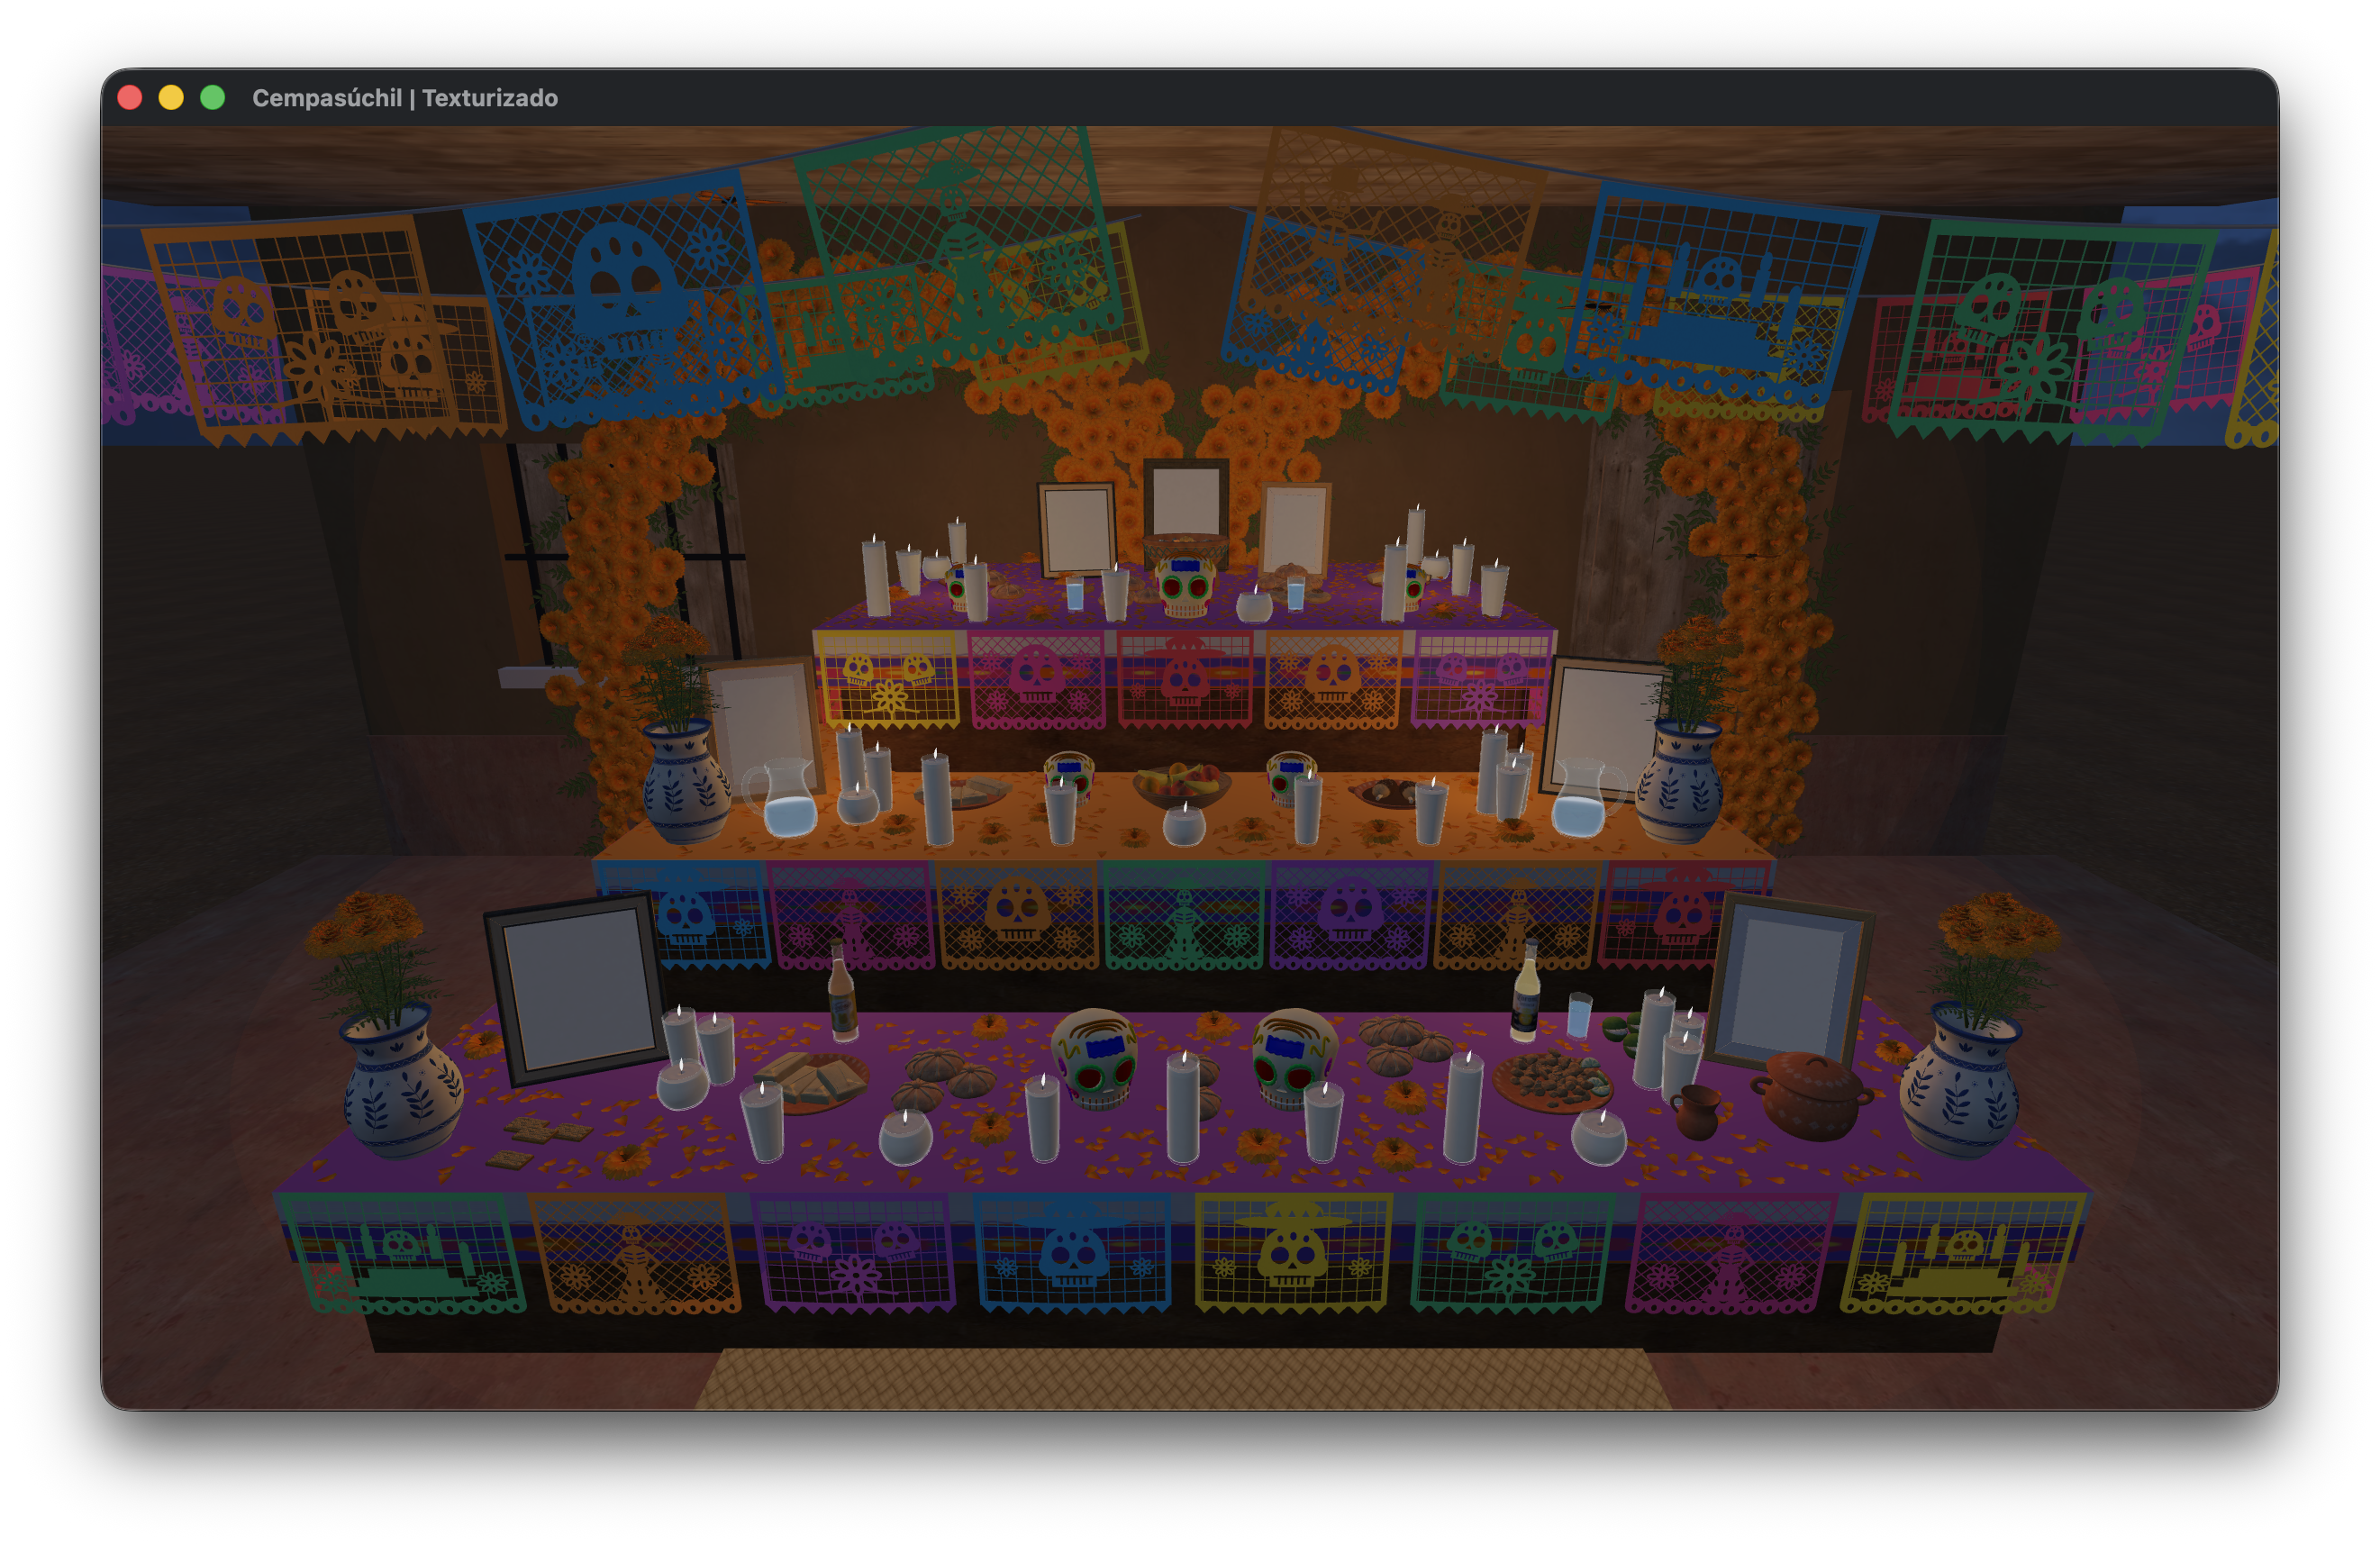
\includegraphics[width=0.85\textwidth]{images/vista-general-ofrenda.png}
		\caption{General view of the illuminated altar.}
	\end{figure}
	
	\begin{figure}[H]
		\centering
		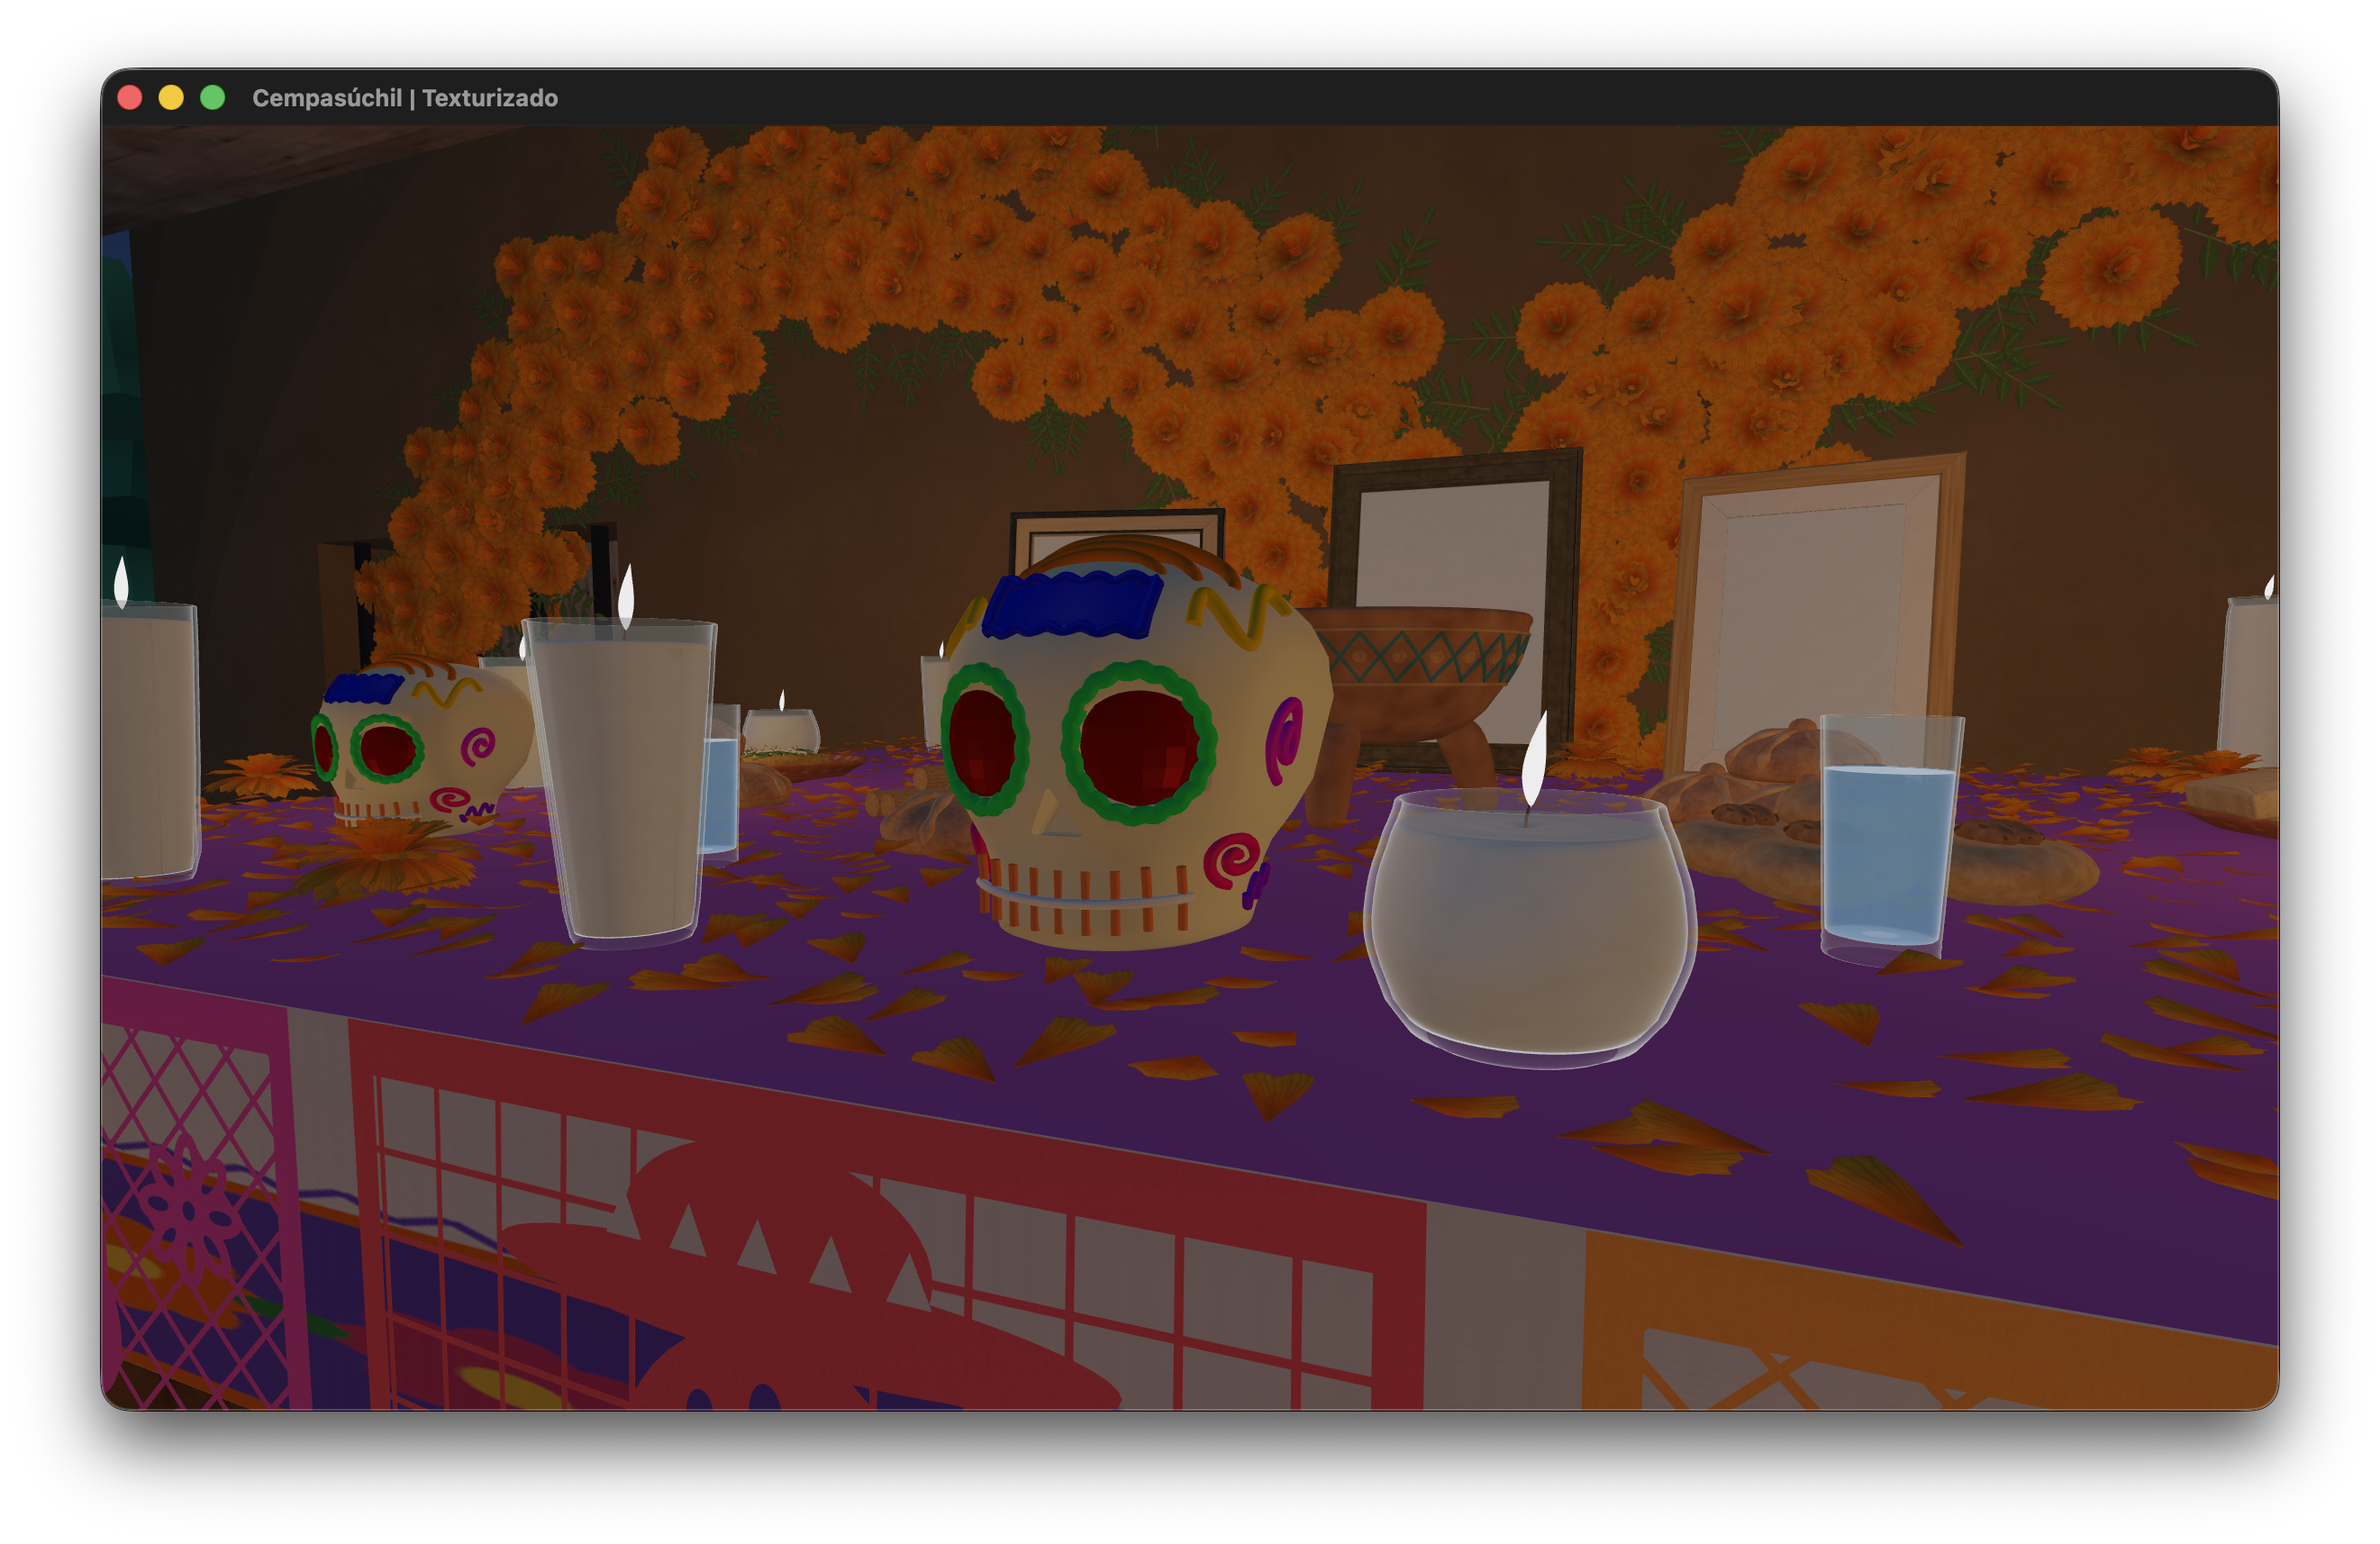
\includegraphics[width=0.85\textwidth]{images/detalle-PBR.png}
		\caption{Detail of PBR textures and point light effect on objects.}
	\end{figure}
	
	\begin{figure}[H]
		\centering
		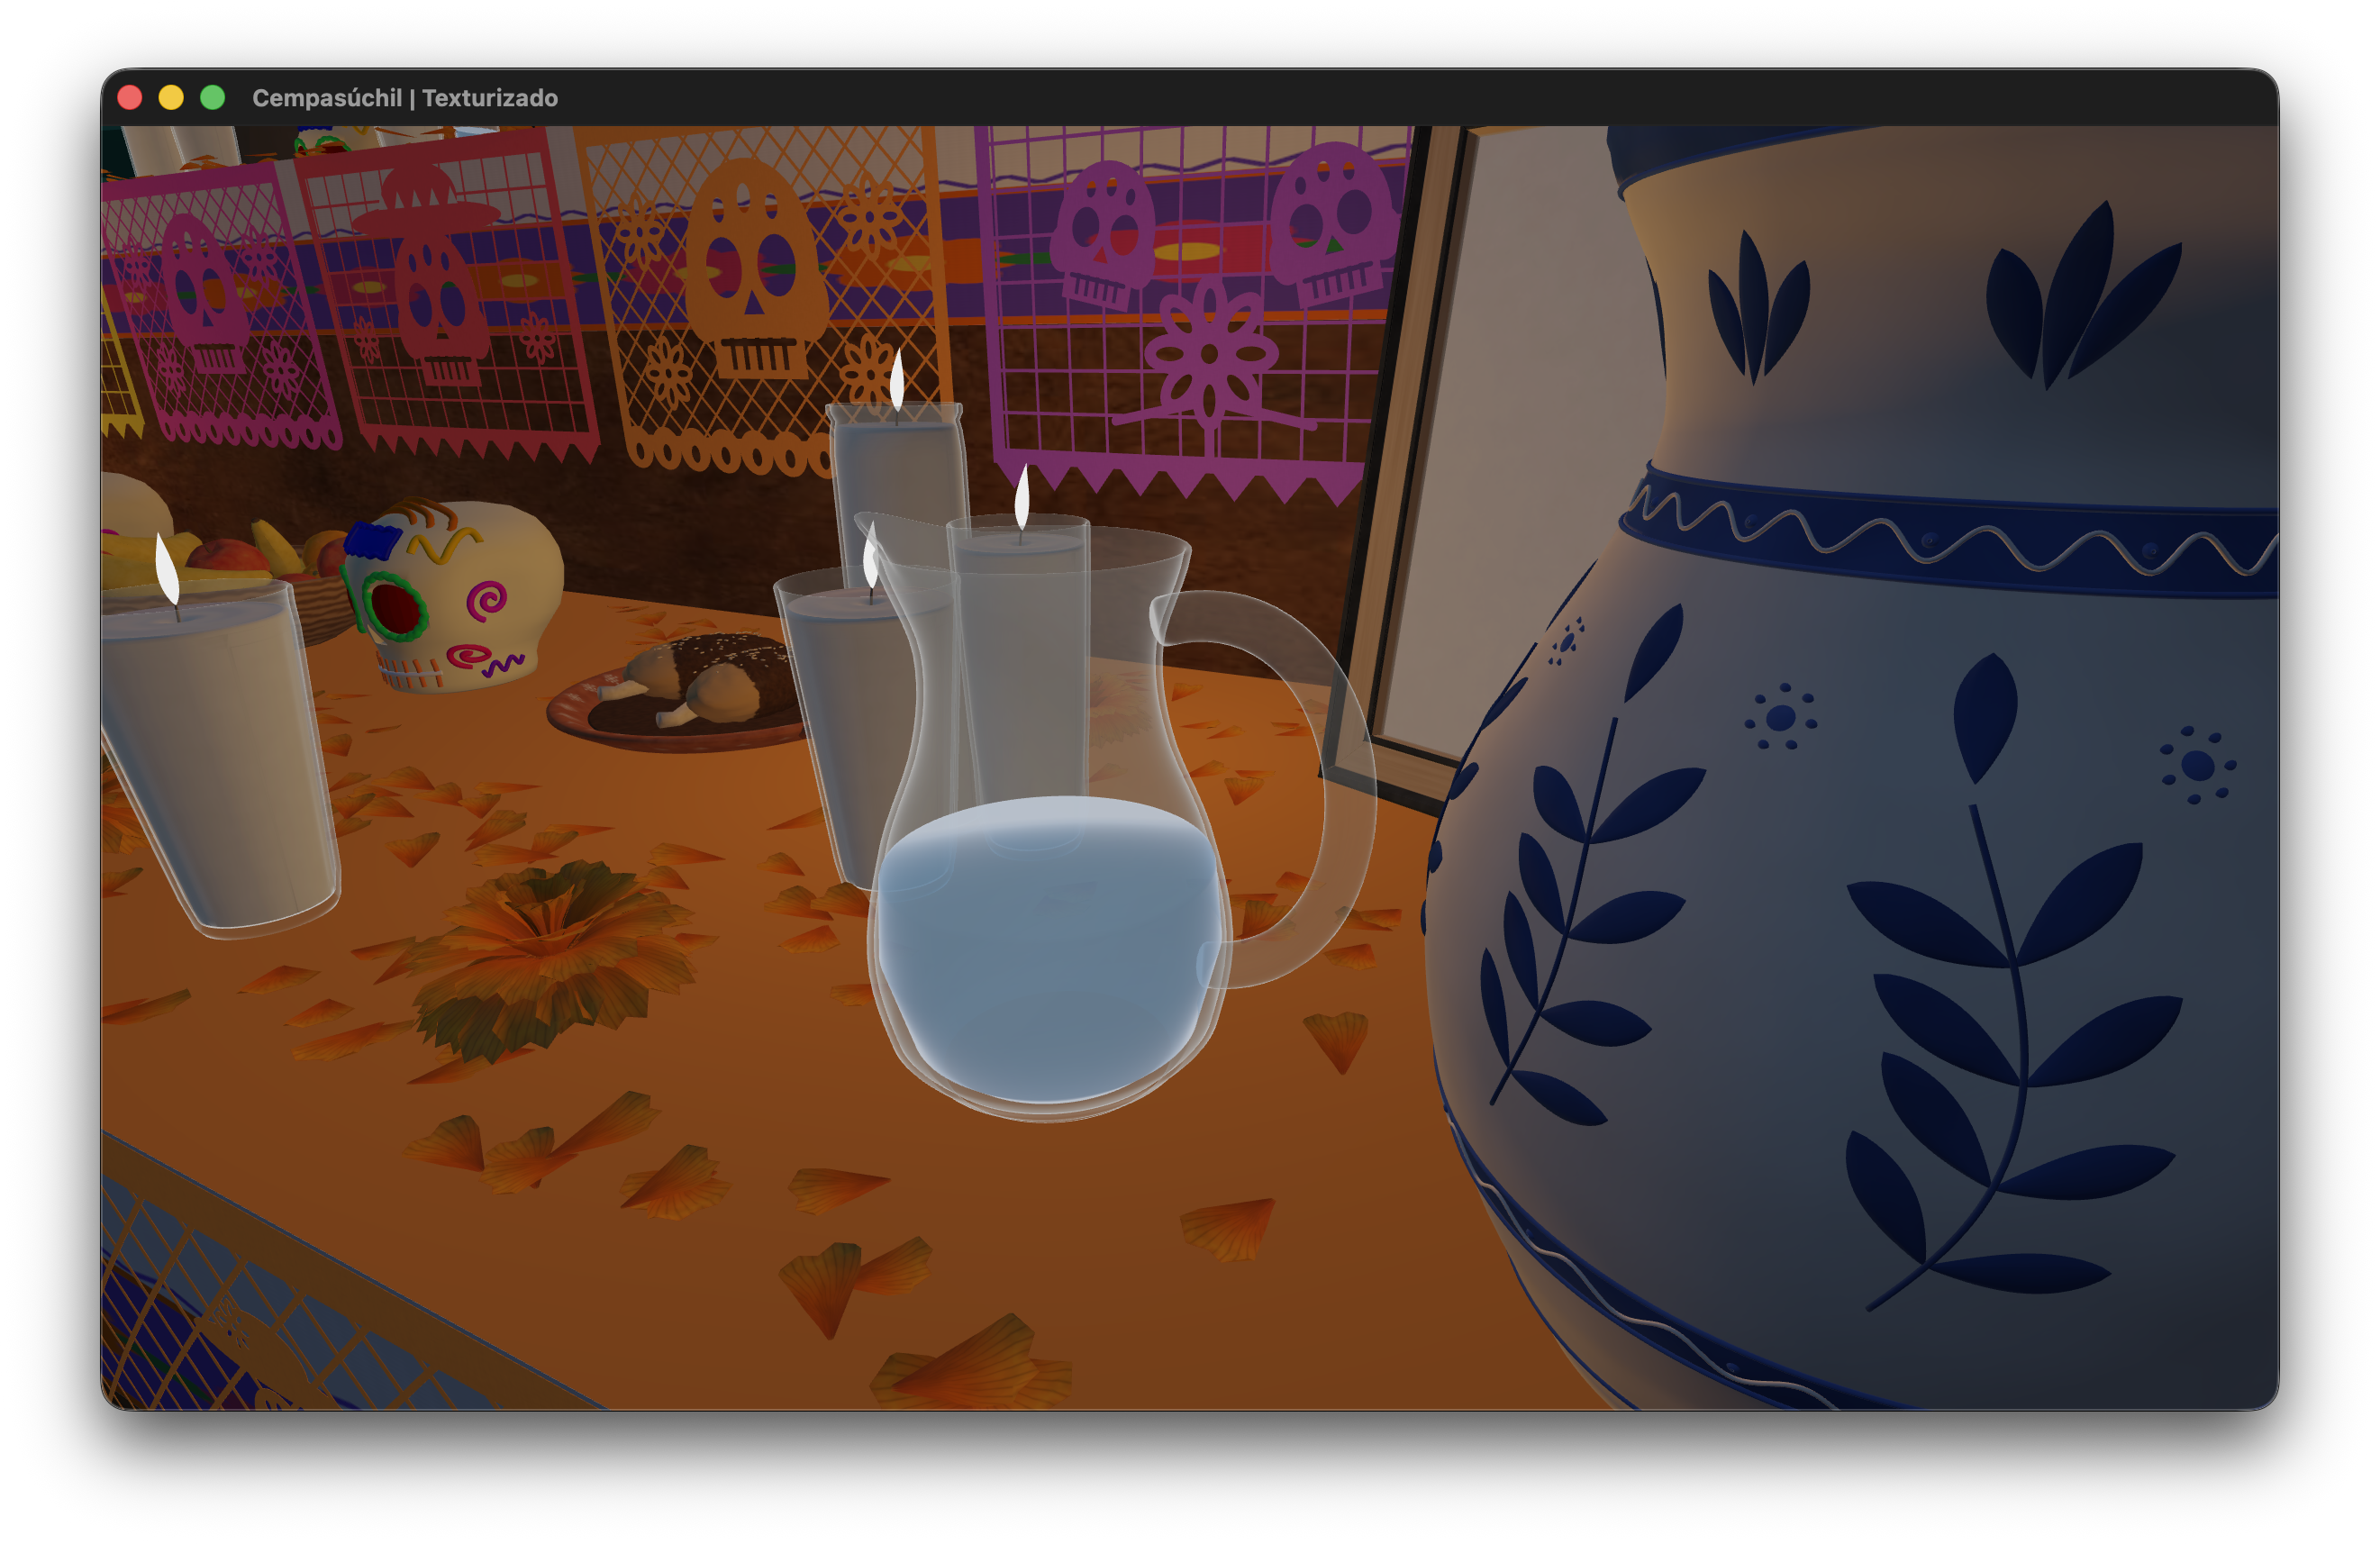
\includegraphics[width=0.85\textwidth]{images/fresnel-1.png}
		\caption{Optical approximation in glass and liquid materials.}
	\end{figure}
	
	\begin{figure}[H]
		\centering
		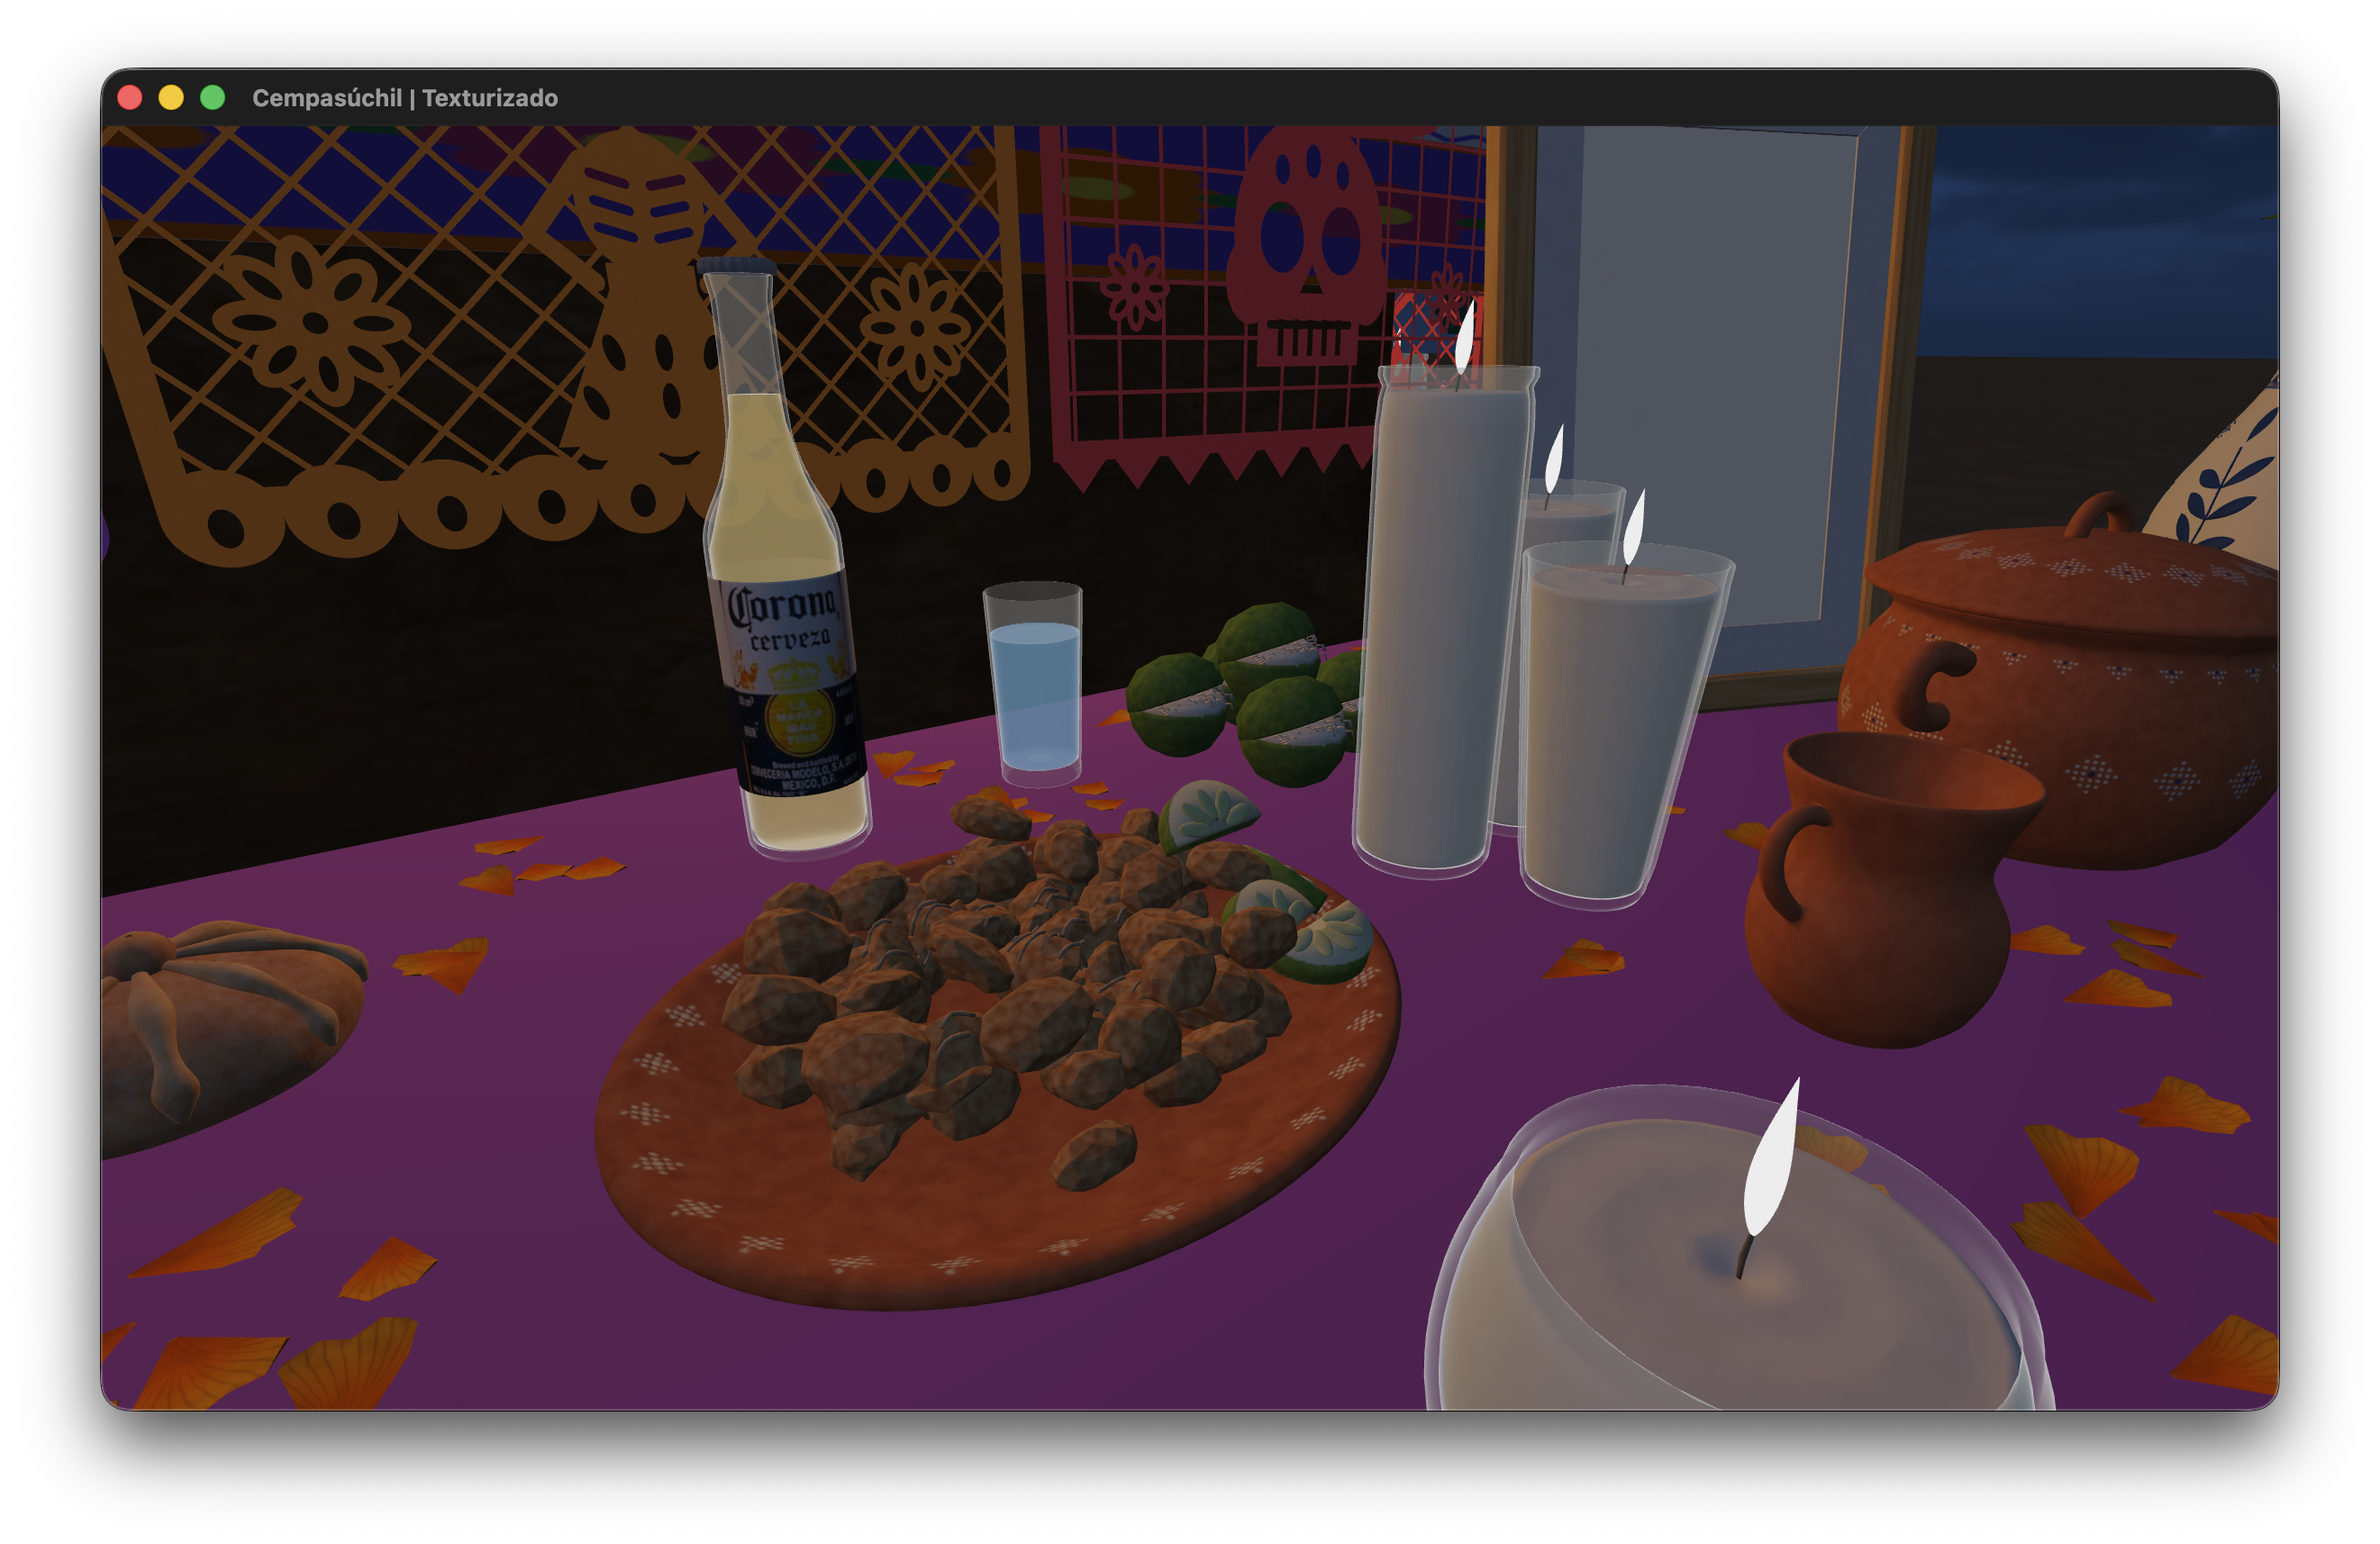
\includegraphics[width=0.85\textwidth]{images/fresnel-2.png}
		\caption{Optical approximation in glass and liquid materials.}
	\end{figure}
	
	\begin{figure}[H]
		\centering
		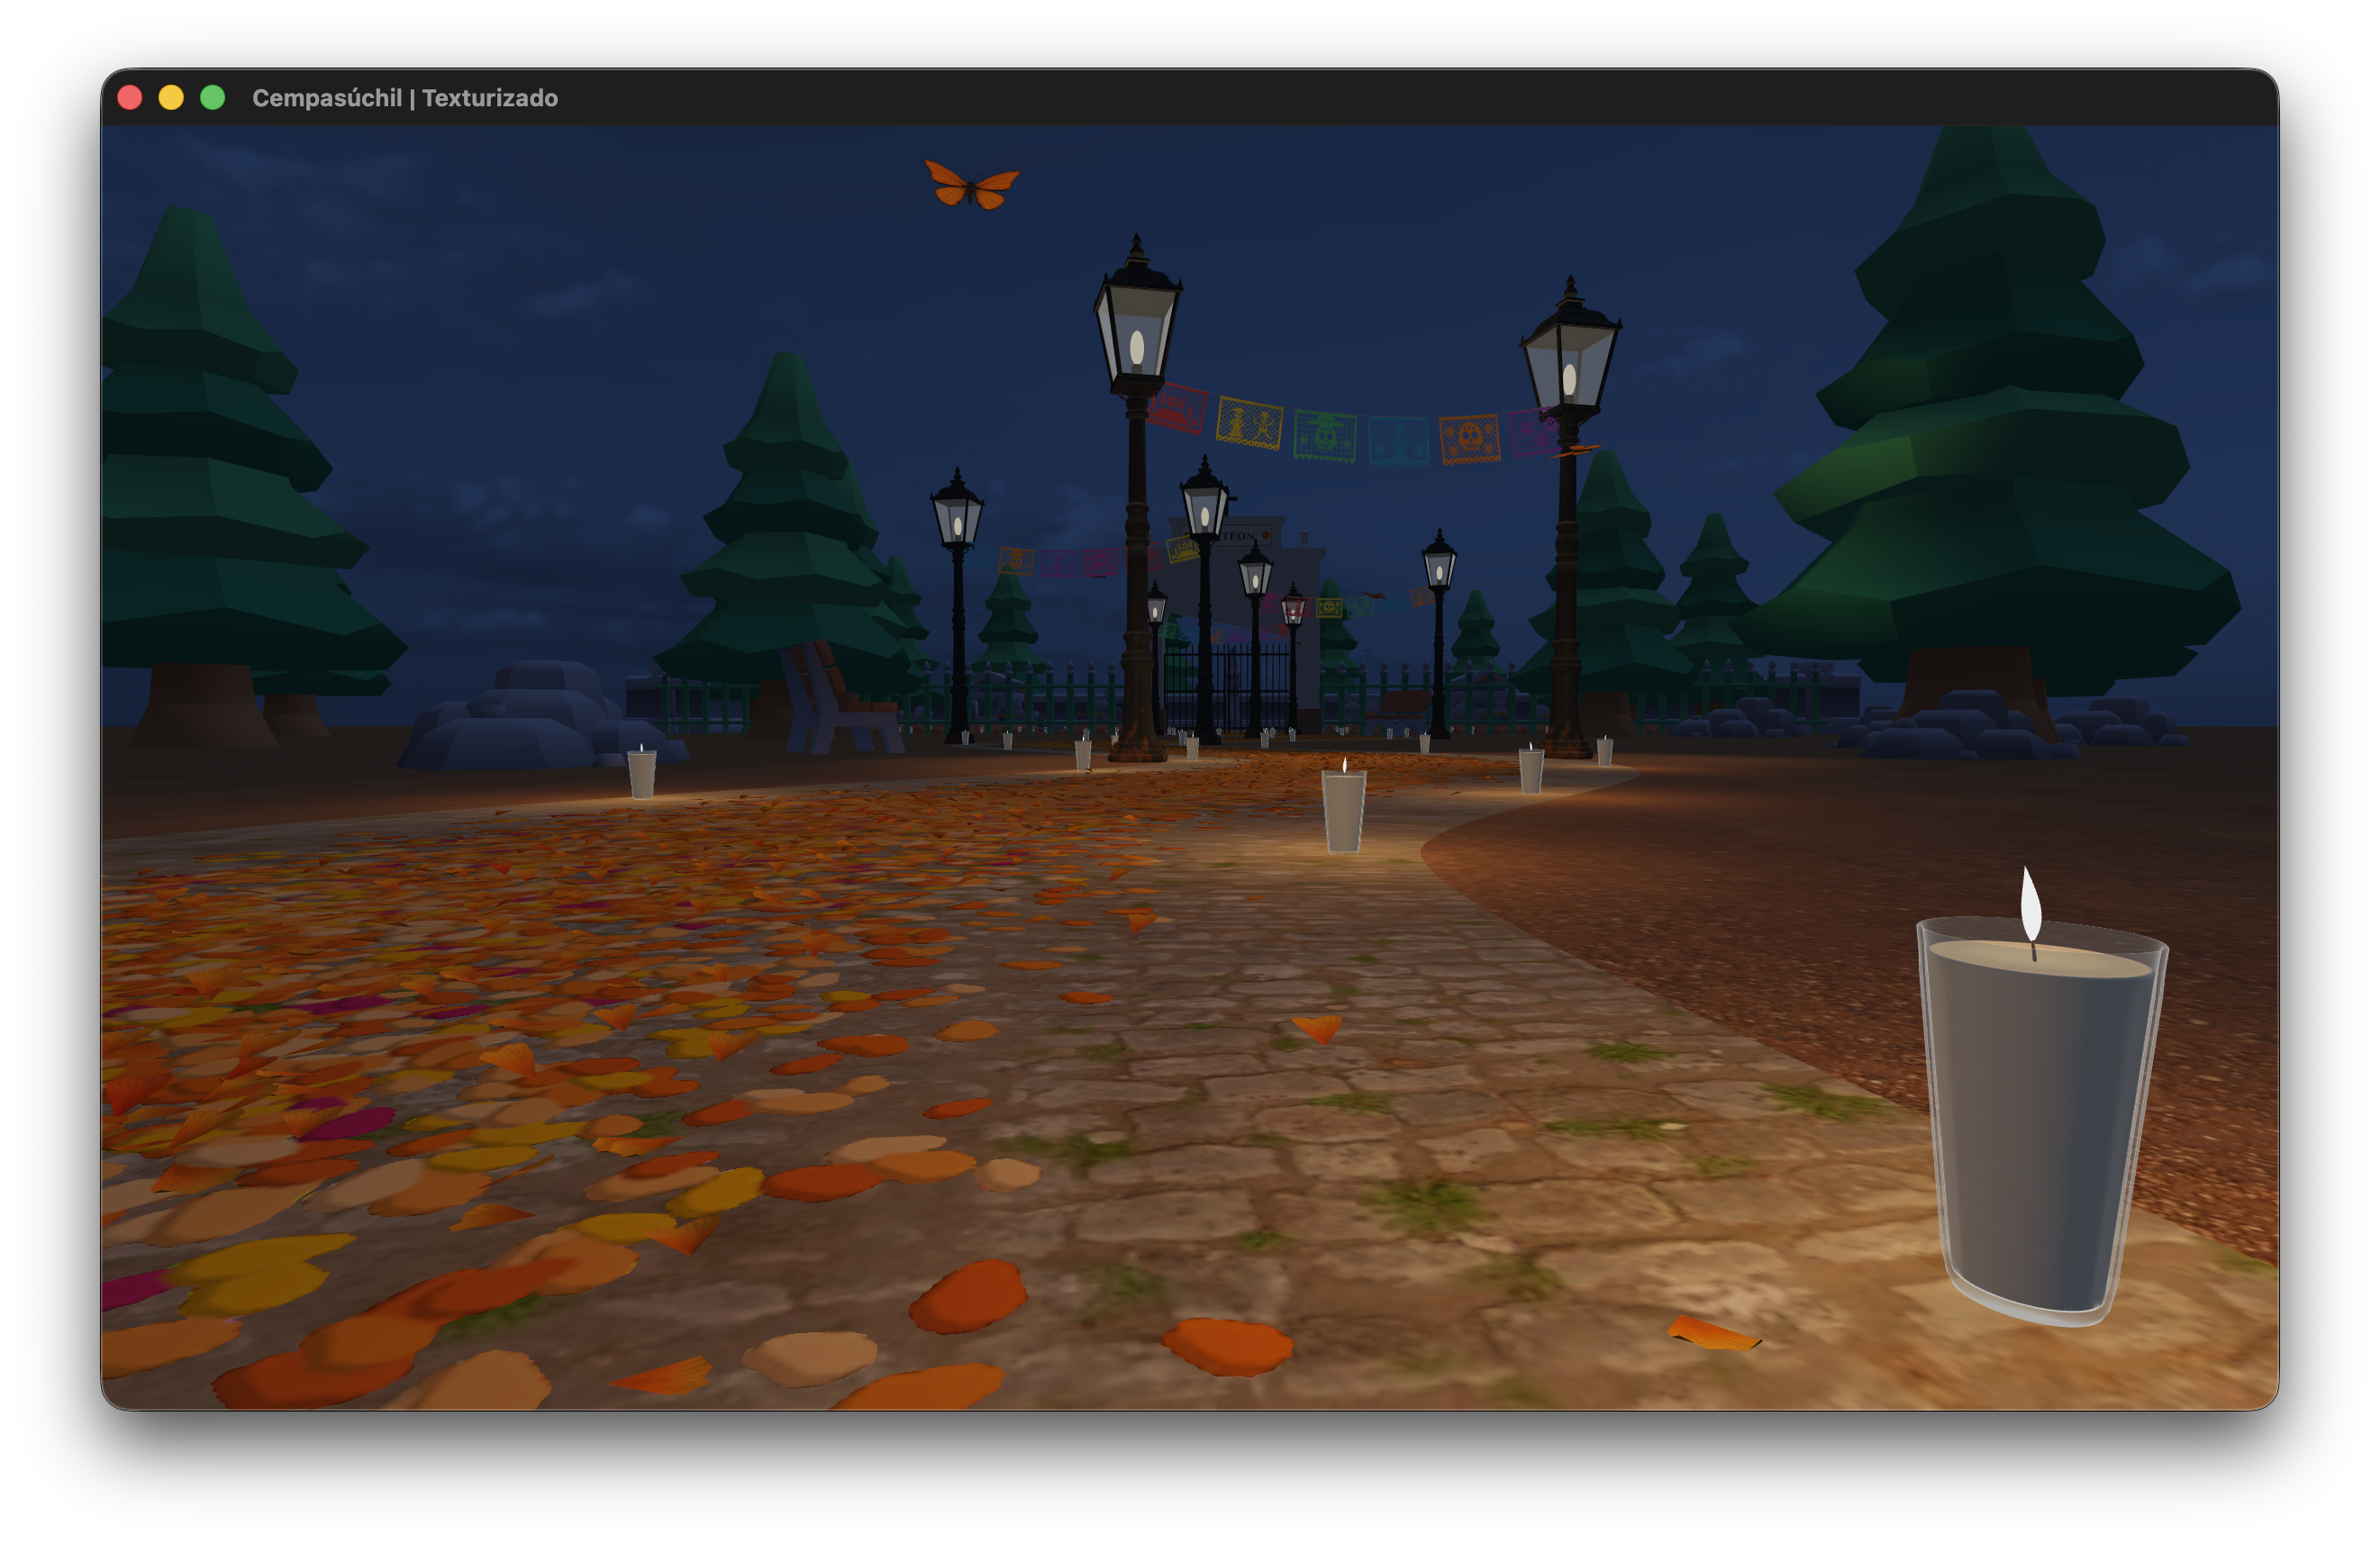
\includegraphics[width=0.85\textwidth]{images/camino.png}
		\caption{Procedural cobblestone path illuminated by lanterns and candles.}
	\end{figure}
	
	\begin{figure}[H]
		\centering
		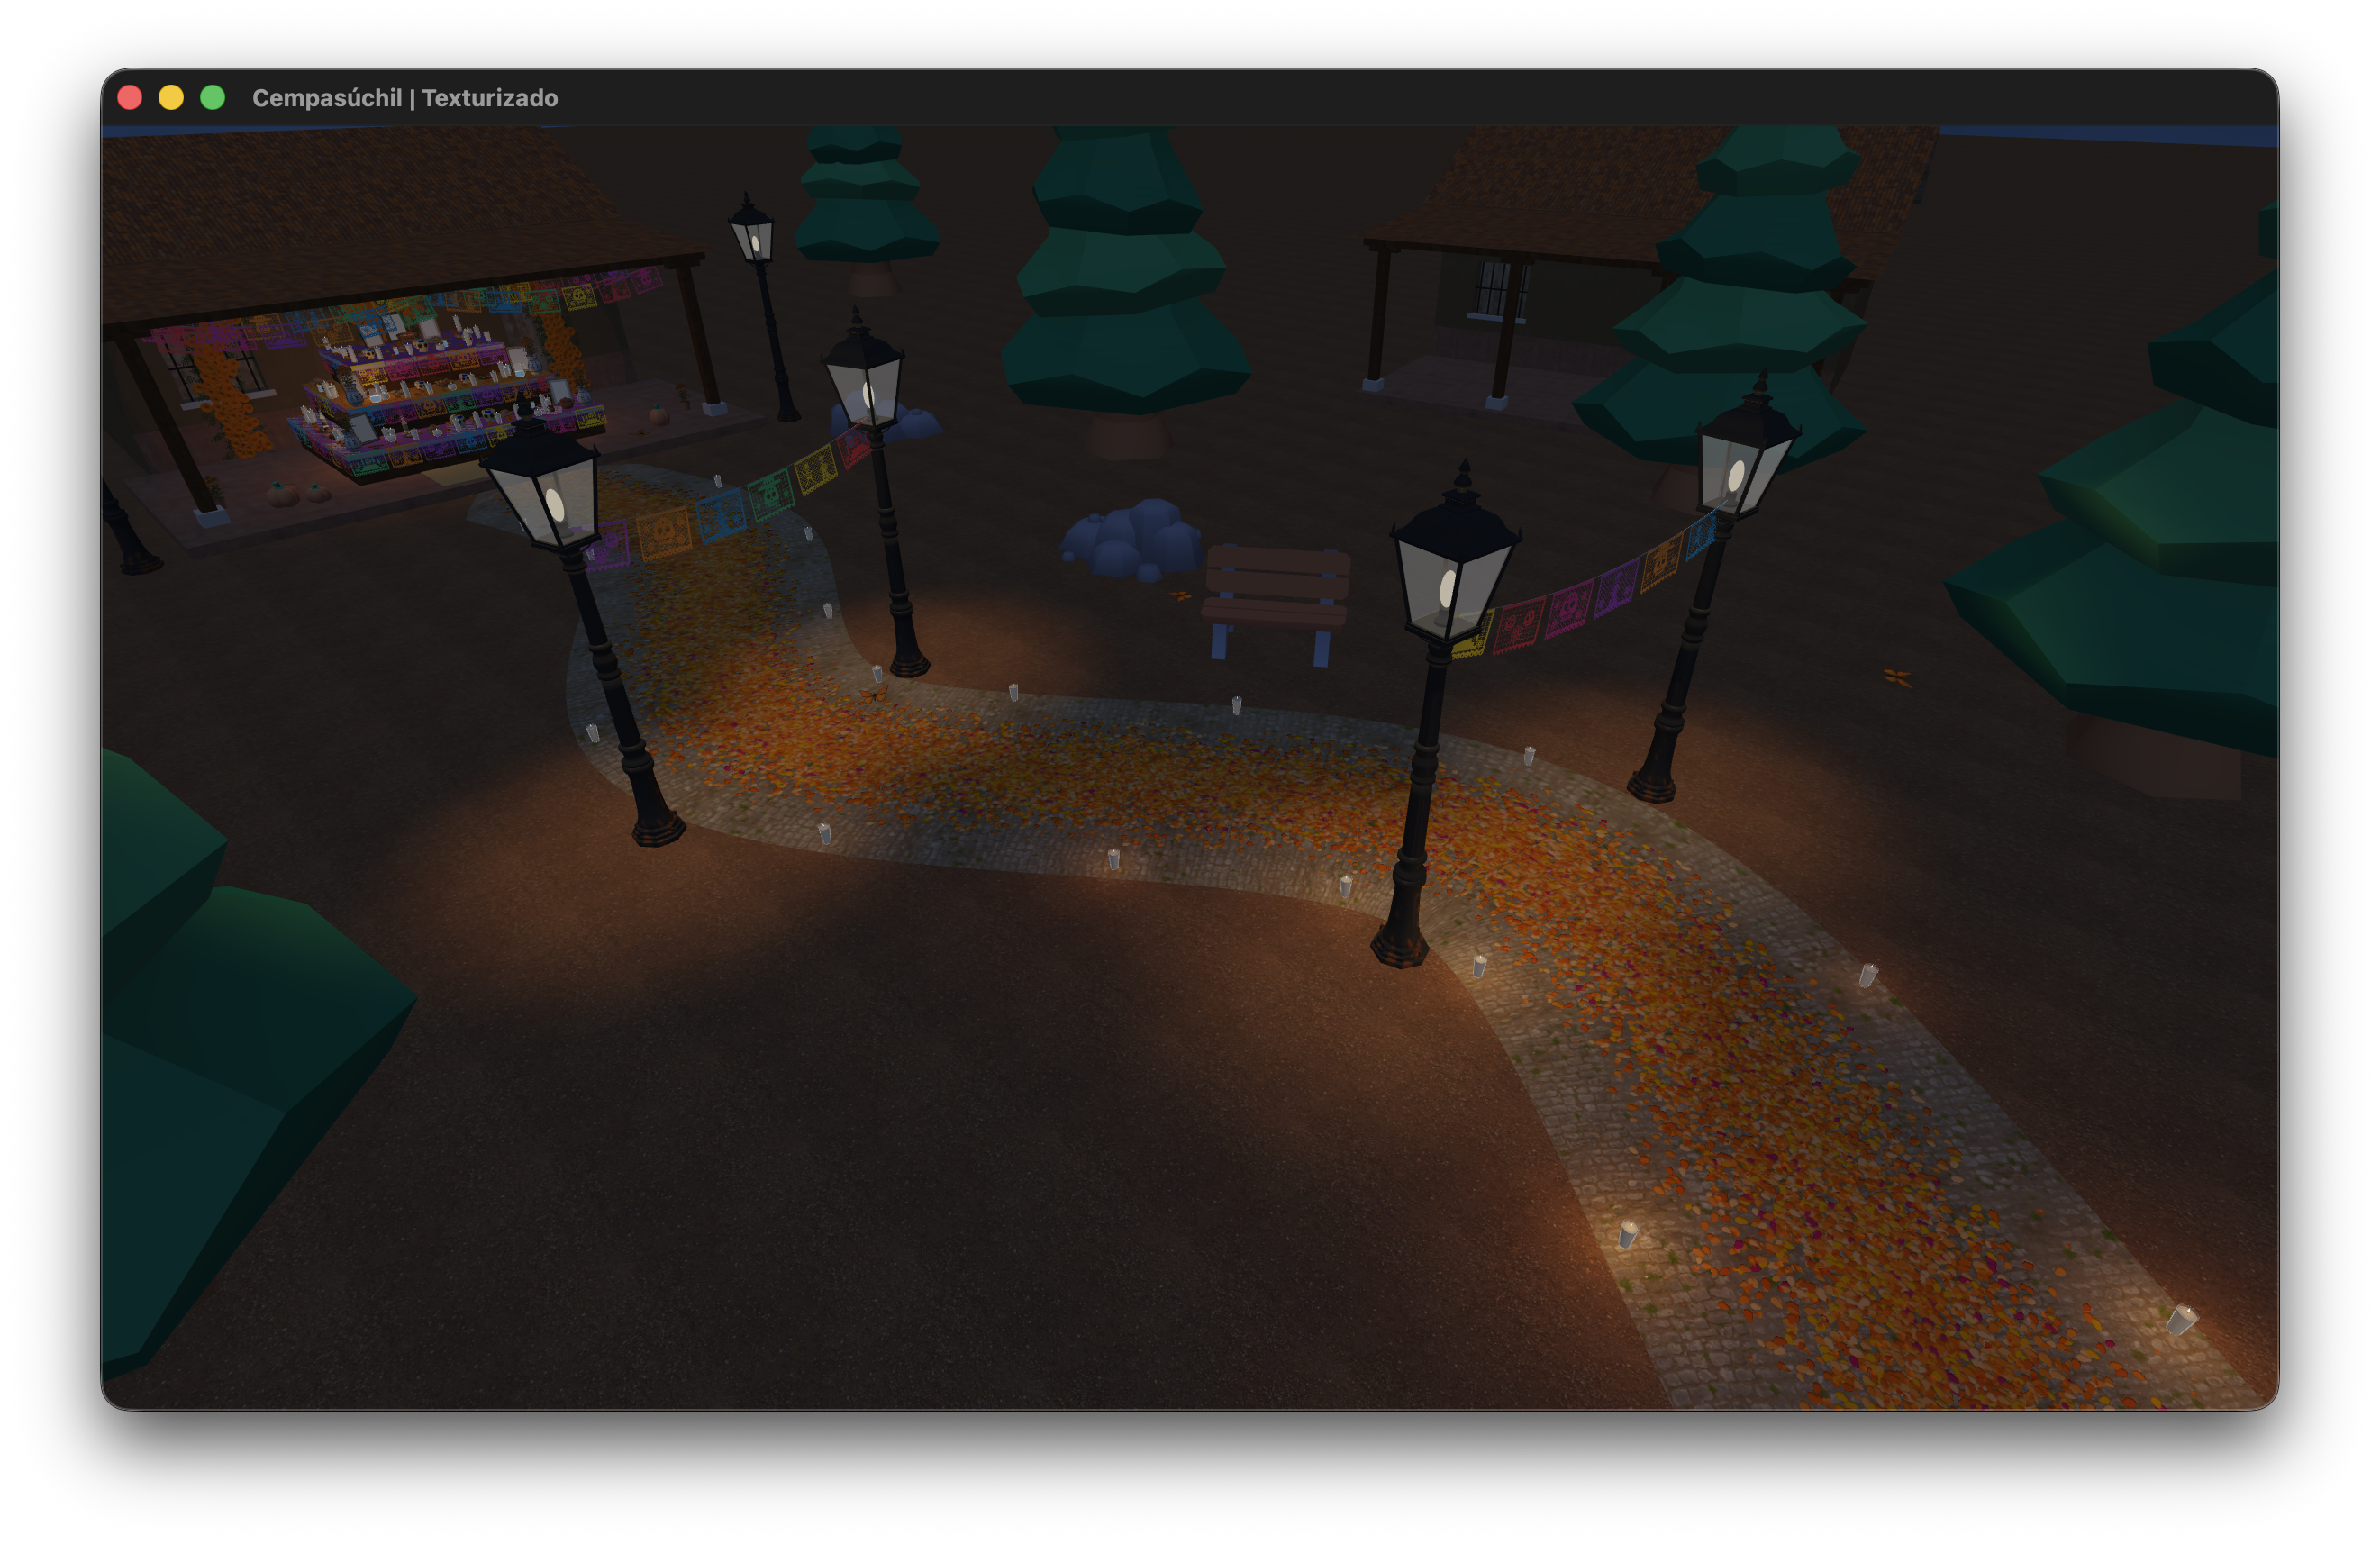
\includegraphics[width=0.85\textwidth]{images/camino-general.png}
		\caption{General view of the illuminated path.}
	\end{figure}
	
	
	\section{Compilation and Execution}
	Execution was validated on macOS, physical Windows, and Linux. Every platform requires a GPU or driver that exposes OpenGL 3.3; 3D or DirectX acceleration alone does not satisfy this requirement.
	
	To optimize the workflow and facilitate project review, the team developed native launchers for each operating system. These shortcuts completely automate the build and deployment cycle, standardizing the process under the following features:
	
	\begin{itemize}[leftmargin=1cm]
		\item Configure and compile the project via CMake strictly in \texttt{Release} mode.
		\item Update and synchronize the resource directories (\texttt{assets} and \texttt{shaders}) into the output directory.
		\item Automatically execute the scene once compilation is finished without running terminal processes.
		\item Keep the console hidden during the process to offer a clean graphical experience.
		\item Redirect and write all technical output, warnings, and diagnostics into the \texttt{logs/} folder located at the root of the project.
	\end{itemize}
	
	\subsection{Launchers by Platform}
	The repository must reside in a local writable directory because each launcher creates a \texttt{build-*} directory. Launchers do not download dependencies and are stored under \texttt{ejecutables/}.
	
	\subsubsection{macOS}
	CMake, Xcode Command Line Tools, and system OpenGL 3.3 support are required. After cloning or downloading the repository, open:
	\begin{lstlisting}[style=terminal]
ejecutables/macOS/TexturizadoCempasuchil-0.2.1.app
	\end{lstlisting}
	Because this local academic application is unsigned, Gatekeeper may block the first attempt; right-click it and select \textbf{Open}. The launcher searches for CMake in \texttt{PATH}, Homebrew, and the official CMake application, builds under \texttt{build-mac-app/}, and retains the last valid binary if a later rebuild fails.

	\subsubsection{Windows}
	Requirements are 64-bit Windows, a GPU driver with OpenGL 3.3, CMake in \texttt{PATH}, and Visual Studio Community 2022 or 2026 with the \textbf{Desktop development with C++} workload, x64/x86 MSVC tools, and a Windows SDK. Then open:
	\begin{lstlisting}[style=terminal]
ejecutables\windows\TexturizadoCempasuchil.vbs
	\end{lstlisting}
	VBScript starts PowerShell without a console; \texttt{vswhere} selects the installed generator and targets x64 under \texttt{build-windows-vs17/} or \texttt{build-windows-vs18/}. Windows ARM64 can cross-compile the x64 executable, but execution still requires a compatible OpenGL driver.

	\subsubsection{Linux}
	CMake, a C++17 compiler, OpenGL, and the X11 development packages used by GLFW are required. Debian/Ubuntu-based distributions can prepare the environment with:
	\begin{lstlisting}[style=bashstyle,numbers=none]
sudo apt update
sudo apt install build-essential cmake libgl1-mesa-dev \
    xorg-dev
	\end{lstlisting}
	On Arch Linux use the equivalent \texttt{base-devel}, \texttt{cmake}, \texttt{mesa}, and \texttt{libx11} packages. Mark the \texttt{.desktop} file as trusted/executable and open it, or run:
	\begin{lstlisting}[style=bashstyle,numbers=none]
chmod +x ejecutables/linux/iniciar_linux.sh
./ejecutables/linux/iniciar_linux.sh
	\end{lstlisting}

	\subsection{Logs and Diagnostics}
	The platform logs are \path{logs/lanzador-macos.log}, \path{logs/lanzador-windows.log}, and \path{logs/lanzador-linux.log}. Internal scene messages are stored as \path{registro.txt} in the build directory. If the application reports that it cannot create a window, check the OpenGL version and update the vendor GPU driver; reinstalling the compiler does not repair a graphics limitation.
	
	\vspace{0.4cm}
	\textbf{NOTE:} For further details on the internal workings of these automated launchers, to review the exact dependencies of each system, or to check the location of the log and diagnostic files, it is highly recommended to read the \texttt{README.md} file located at the \texttt{ejecutables/README.md} path.
	
	\section{Results and Conclusions}
	The texturing and lighting phase significantly elevated the visual impact and immersion of the Day of the Dead environment. However, implementing the hybrid lighting model presented a major performance challenge for the team. By integrating dynamic light sources, we detected severe bottlenecks because some models exported from Blender had an excessive polygon density; the graphics engine was calculating lighting per fragment over an unnecessary amount of triangles, saturating the processing pipeline. The implemented solution was to optimize these models, drastically reducing their triangle count (retopology and decimation) while retaining a visual appearance practically identical to the original thanks to the detail provided by the normal maps.
	
	The use of procedurally crafted PBR textures, coupled with normal calculations derived directly in the \textit{fragment shader}, demonstrated an excellent balance between photographic quality and algorithmic optimization. Likewise, the cross-platform architectural design was crucial in successfully overcoming technical barriers related to native libraries, file systems, repositories, and high-resolution interfaces.
	
	Proper alpha mapping to reduce polygons (as seen in the petal carpet), geometric optimization of the meshes, and the simulated refraction system allow us to affirm that the delivery satisfactorily meets the proposed visual parameters. For the final phase, the robust and optimized technical environment built so far will serve as an ideal foundation to seamlessly integrate particle systems and animations.
	
	\section{References}
	\begin{itemize}[leftmargin=*]
		\item Blender Foundation. (2026). \textit{Blender 5.2}. \url{https://www.blender.org/}
		\item Khronos Group. (2021). \textit{glTF 2.0 Specification}. \url{https://registry.khronos.org/glTF/specs/2.0/glTF-2.0.html}
		\item Khronos Group. (2010). \textit{OpenGL 3.3 Core Profile Specification}. \url{https://registry.khronos.org/OpenGL/specs/gl/glspec33.core.pdf}
		\item Kitware. (2026). \textit{CMake Documentation}. \url{https://cmake.org/documentation/}
		\item nothings/stb. (2025). \textit{stb\_image 2.30}. \url{https://github.com/nothings/stb}
		\item GLFW. (2026). \textit{GLFW Documentation}. \url{https://www.glfw.org/documentation.html}
	\end{itemize}
\end{document}
